
\documentclass[conference]{IEEEtran}
\usepackage[utf8]{inputenc}
\usepackage{graphicx}
\usepackage{amsmath}
\usepackage{amssymb}
\usepackage[version=4]{mhchem}
\usepackage{siunitx}
\usepackage{longtable,tabularx}
\usepackage{listings}
\usepackage{float}

%\usepackage{subcaption}
\usepackage{multicol}
\usepackage{dblfloatfix}
\usepackage{color}
\usepackage{subfigure}% subcaptions for subfigures
\usepackage{subfigmat}% matrices of similar subfigures, aka small
%\hyphenation{op-tical net-works semi-conduc-tor}
\usepackage{multirow}
\usepackage[table,xcdraw]{xcolor}
\usepackage{soul}

%\floatstyle{boxed}
%\restylefloat{figure}




\begin{document}

\title{An Intercept and Following Strategy for a Multi-rotor Platform using a Modified Proportional Navigation}

\author{\IEEEauthorblockN{Garrett S. Clem, Jay P. Wilhelm}
\IEEEauthorblockA{Department of Mechanical Engineering\\
Ohio University\\
Athens, Ohio 45701\\
Email: gc117711@ohio.edu, jwilhel@ohio.edu}
\and
\IEEEauthorblockN{David Casbeer, David Grymin, Isaac Weintraub}
\IEEEauthorblockA{AFRL RQQA\\
AFRL\\
Wright-Patterson Air Force Base, Ohio 45433\\
Email: david.casbeer@us.af.mil, grymin, isaacweintraub.1@us.af.mil}
}

\maketitle


\begin{abstract}
	Combatant small Unmanned Aerial Vehicles (CUAVs) can easily enter restricted airspace and may be mitigated by counter UAVs. Intercepting and following combatant UAVs in restricted airspace could be achieved with multi-rotor UAVs. A pseudotarget based proportional navigation (PN) guidance algorithm that guides a UAV to intercept and follow a combatant UAV using highly uncertain sensor position information was investigated. Simulations were performed to validate the model and develop a ratio of following distance to initial range. Near zero following distance was achieved for a finite range of initial line-of-sight angles.
\end{abstract}

\begin{IEEEkeywords}
	UAV
	Multi-rotor
	Fixed Wing
	Guidance
	Proportional Navigation
	Uncertainty

\end{IEEEkeywords}

\section{Introduction}
%==========Motivation ============

Tracking and following small unmanned systems (sUAS) have applications in autonomous flight formation, swarming, and standoff target tracking. Multi-rotor sUAS may also be guided to passively track and follow another target sUAS flying in restricted airspace. Path planning, heading control laws, and line-of-sight (LOS) guidance algorithms have been proposed for intercepting and following moving targets. Path planning is typically performed at a ground station requiring constant communication to adapt for a moving target. Control laws for target tracking rely on low uncertainty target position estimates. Line-of-sight methods such as proportional navigation (PN) guidance have been used in missile systems to track targets but may fail to follow a target under head-on intercept scenarios. Direction and range to the target can be measured with on-board sensors but provide highly uncertain estimates due to limitations in the sensing technology. \\

A pseudotarget PN guidance algorithm that directs a sUAS to intercept and follow a target sUAS using uncertain position information was investigated. First the interceptor and target kinematics are presented along with the unmodified PN guidance algorithm. Next an on-board sensor that measures the target's position, which has some uncertainty, is modeled. A state machine pseudotarget is than introduced that intercepts and follows a target with high initial position uncertainty for head-on and tail-chase scenarios. Simulations were performed to validate the model and to show that the following distance can be predicted from the initial LOS angle, range, and sensor characteristic.

%Multi-rotor sUAS may be guided to passively track and follow another small Unmanned Aerial Systems (sUAS). On-board direction and ranging sensor technology for sUAS currently only provides a highly uncertain position estimation. Proportional navigation guidance has been used by missiles to track targets. PN guidance may be useful for guiding a mutli-rotor sUAS to intercept and follow other sUAS. Interception and following has applications in autonomous flight formation and swarming scenarios as well. The objective was to use a modified PN guidance to track other sUAS with uncertain position information.


\subsection{Literature}
% ======= Literature =========
Tracking an aerial target has been achieved by implementing closed-loop feedback systems, path following guidance, and line-of-sight (LOS) guidance algorithms. Closed-loop position and velocity control of a multi-rotor for following a ground target with intermittent and noisy vision data was achieved in \cite{teuliere_chasing_2011}. Vision systems suffer from field of view distance limitations and are sensitive to differential lighting conditions. Following time varying paths and intercepting multiple ground targets was demonstrated in \cite{oliveira_moving_2016} by introducing a heading control law. Distance to the target at interception varied an order of magnitude and required knowledge of targets position. 

Target tracking without modification of a UAVs control system has been accomplished by framing target tracking as a path planning problem. A waypoint generation technique was developed in \cite{ariyur_autonomous_2008} that satisfied fixed wing forward velocity constraints while maintaining the target in the field-of-view. Sub-optimal placement of waypoints resulted in exaggerated trajectories for fixed wings when tracking an accelerating target. Multi-rotors tracked the target with less error when navigating waypoints for the same scenario due to the multi-rotors ability to hover. Less exaggerated trajectories for tracking a maneuvering target was accomplished for a fixed wing UAV in \cite{lee_strategies_2003}.  An optimal path planning strategy consisting of a Markov Decision Process and cost based state reduction showed less tracking error in comparison to lookup tables and heuristic methods, but took considerably longer to provide a solution \cite{baek_optimal_2013}. Target tracking with path planning techniques may require the UAV to be in constant contact with the ground station where planning typically occurs.  

Target tracking may also be accomplished by implementing line-of-sight (LOS) guidance methods, such as those used in missiles \cite{zarchan}. LOS methods control the missile’s velocity to be on a collision triangle with the target \cite{shneydor1998missile,yanushevsky2007modern}. Adapting a pure pursuit line-of-sight (LOS) guidance to chase a target with less tracking error than traditional pure pursuit guidance was demonstrated in \cite{yamasaki_advanced_2009}.  Proportional navigation (PN) guides a missile to a target by nulling the line-of-sight (LOS) rate \cite{shneydor1998missile}-\cite{yanushevsky2007modern}. PN guidance has had continued interest and may have new uses such as cooperative defense strategies \cite{isaac}. The PN guidance law controls a missile to intercept a target but does not contain arguments to command a specific approach angle. Ratnoo and Ghose modified the PN guidance gain throughout flight to satisfy a terminal angle constraint \cite{ratnoo2009satisfying}. Oza and Padhi discuss how time varying guidance gains result in singularities near the end of the flight and provide an impact-angle-constrained suboptimal model predictive static programming guidance \cite{oza2012impact}. Optimal impact-angle-constrained guidance algorithms have been developed for 2D \cite{park2013optimal} and 3D \cite{kumar2014three} engagements. The impact-angle constrained guidance in literature have additional levels of complexity in comparison to traditional PN guidance and may be more complicated to implement. Achieving a terminal angle constraint can be accomplished without modifying the PN guidance gain or implementing an entirely new guidance model by introducing a pseudotarget into the engagement scenario.



%\subsection{Methods}
%Interceptor and target kinematics are first presented, followed by the traditional PN guidance law. Next an on-board sensor that measures the target's position, which has some uncertainty, is modeled. A state machine pseudotarget is introduced that prevents the intercepting UAV from entering the uncertain area while accomplishing the main goal of intercepting and following the target. Simulations were performed to validate the model and to show that the following distance can be predicted from the initial LOS angle, range, and sensor characteristic.

\section{Model}

\subsection{Intercept Model}
An interceptor and target were modeled as Dubins vehicles in $\mathbb{R}^2$ with $x$ representing East and $y$ altitude, shown in Figure \ref{fig:Egagement}. UAV position $[x \quad y]^T$ was determined from the integral of the velocity $[\dot{x} \quad \dot{y}]^T$ shown in Equation \ref{eq:dubinUAV}. The heading of both sUAS was the input $u$ and was bounded on the interval $[0,2\pi)$. The non-maneuvering target heading $\beta$ was a constant while interceptor heading $\gamma$ was determined by PN guidance. The line-of-sight angle $\lambda$ is the angle between the interceptor and target with respect to the positive $x$ axis. 



\begin{equation} \label{eq:dubinUAV}
\begin{split}
\dot{x} = v\cos(\phi)\\
\dot{y} = v\sin(\phi)
\end{split}
\end{equation}

\begin{equation}\label{eq:dubinsVel}
\phi = u
\end{equation}
 

\begin{figure}[H]
	\centering
	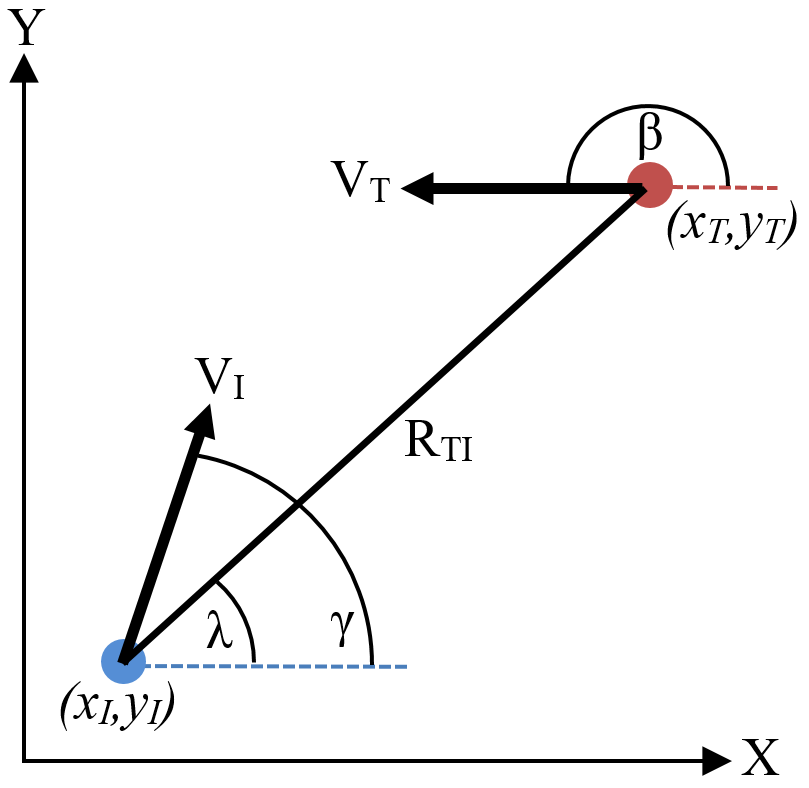
\includegraphics[width=6 cm]{Engagement_Model.PNG}
	\caption{Interceptor and Target Engagement Scenario (x-East, y-Up)}
	\label{fig:Egagement}
\end{figure}

The PN guidance law operates on the principle of proportionally controlling heading so that the line-of-sight rate (LOS) $\dot{\lambda}$ is null. The input rate $\dot{u}$ is proportional to the LOS rate and a fixed guidance gain $N$. Second order Runge-Kutta integration is typically used to determine $u$ from Equation \ref{eq:PNlaw}.

\begin{equation} \label{eq:PNlaw}
\dot{u} = N\dot{\lambda}
\end{equation}


Guidance gains of $N < 3$ are generally referred to as conservative, while $N > 5$ are referred to as more aggressive \cite{zarchan}. Conservative gains result in larger turn radii whereas larger gains result in smaller turn radii. Multi-rotors are capable of making abrupt heading changes in comparison to fixed wing UAVs and it was assumed a guidance gain of $N = 5$ is not beyond multi-rotor capability. The resulting guidance is expected to return sharp turns and straight line optimal paths when used with the Dubins kinematic model. The LOS angle and rate are calculated in Equations \ref{eq:LOS} and \ref{eq:losrate} respectively. Table \ref{relations} summarizes the symbols used.
 
 \begin{table}
 \centering
 \caption{Equation relations}
 \begin{tabular}{cc}
 	\label{relations}

 	$Variable$ & $Relation$ \\
 	\hline 
 	$x_I$  & Interceptor x position \\ 
 	
 	$y_I$ & Interceptor y position \\ 
 	
 	$V_{Ix}$ & Interceptor x velocity \\ 
 	
 	$V_{Iy}$ & Interceptor y velocity \\ 
 	
 	$x_T$ & Target x position \\ 
 	
 	$y_T$ & Target y position \\ 
 	
 	$V_{Tx}$ & Target x velocity \\ 
 	
 	$V_{Ty}$ & Target y velocity \\ 

 \end{tabular}
 \end{table}







\begin{equation} \label{eq:LOS}
\lambda = \tan^{-1} \left(\frac{y_T - y_I}{x_T - x_I}\right)
\end{equation} 

\begin{equation} \label{eq:losrate}
\dot{\lambda} = \frac{(x_T - x_I)(V_{Ty}-V_{Iy}) - (y_T - y_I)(V_{Tx}-V_{Ix})}{(x_T - x_I)^2+(y_T - y_I)^2}
\end{equation}




Range is the Euclidean distance between the target and the interceptor, shown in Equation \ref{eq:range}. 

\begin{equation} \label{eq:range}
R_{TI} =\sqrt[]{(x_T - x_I)^2+((y_T - y_I)^2}
\end{equation}


 


PN guidance is effective at reducing the range between the interceptor and the target, however it does not always setup the interceptor to follow once the range is at a minimum. For head-on intercept shown in Figure \ref{fig:failedIntercept} and \ref{fig:failedInterceptLOS} the LOS rate experiences a singularity and fails to follow the target. The singularity is caused by a combination of relative velocity sign change and division by zero. Solutions around the singularity can be obtained for a linearized proportional navigation \cite{singularitySolution} but are not a concern for traditional missile systems because the mission is complete when the range is near zero. For an intercepting UAV with the intention of following the target, a singularity  calls for control efforts beyond the saturation point. After the singularity occurs there remains a possibility for the nulled LOS condition to be met even if the interceptor and target are heading away from each other. Figure \ref{fig:failedIntercept} demonstrates how for head-on intercepts the nulled LOS rate can be satisfied and the interceptor flys away from the target. Figure \ref{fig:failedInterceptLOS} shows how a singularity can occur near zero range.




\begin{figure}[H]
	\centering
	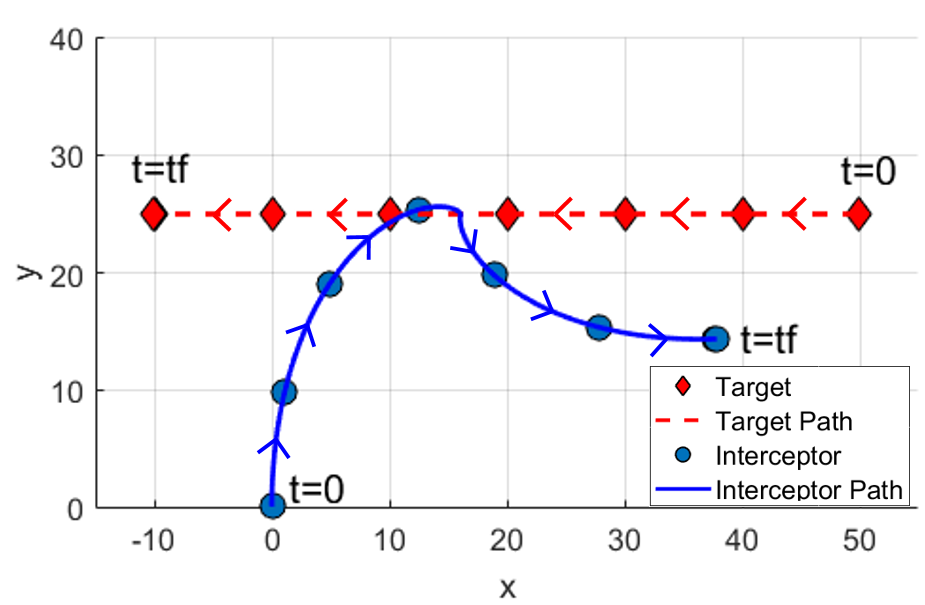
\includegraphics[width=7cm] {failedHeadOn}
	\caption{Failed follow for head on intercept}
	\label{fig:failedIntercept}
	\hspace*{0mm}
\end{figure}


\begin{figure}[H]
	\centering
	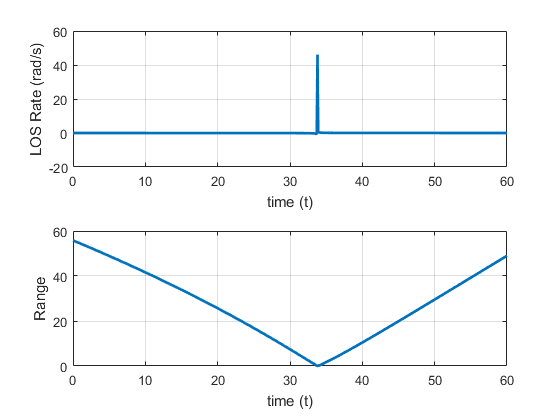
\includegraphics[width=7cm] {x50_range_LOSrate}
	\caption{Failed follow with LOS-rate singularity and range}
	\label{fig:failedInterceptLOS}
	\hspace*{0mm}
\end{figure}


The interceptor successfully intercepts and follow the target for a tail-chase scenario shown in Figure \ref{fig:successfulFollow} and no singularities are present in Figure \ref{fig:successfulFollowLOS}. The tail-chase scenario has the added benefit of placing the interceptor behind the target, allowing for a transition into a follow. The elimination of the singularity and easy transition into a follow make a case for waiting on the target before intercepting it directly, which is the motivation for introducing a pseudotarget into the PN guidance model.

\begin{figure}[H]
	\centering
	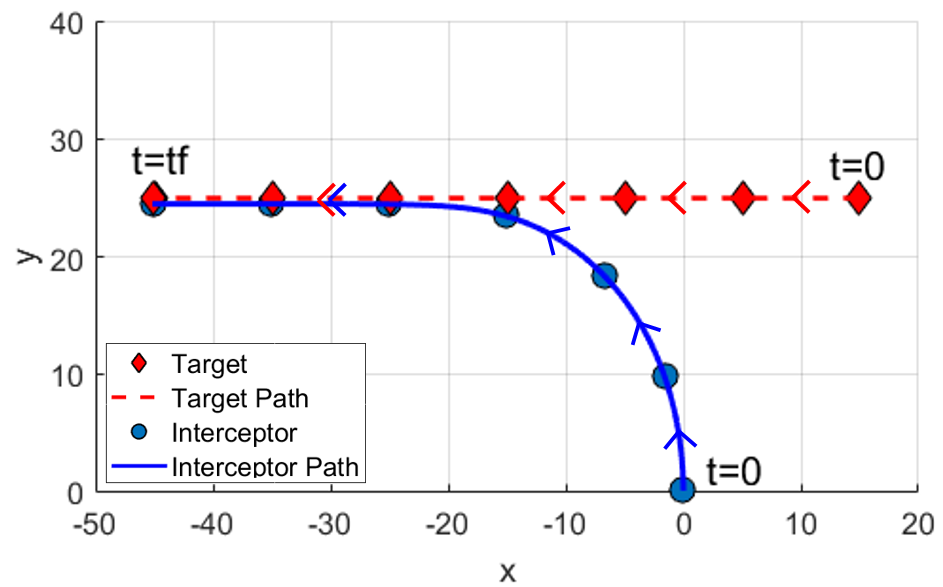
\includegraphics[width=7cm] {tailChaseWithLedgend}
	\caption{Successful follow for tail chase intercept}
	\label{fig:successfulFollow}
	\hspace*{0mm}
\end{figure}

\begin{figure}[H]
	\centering
	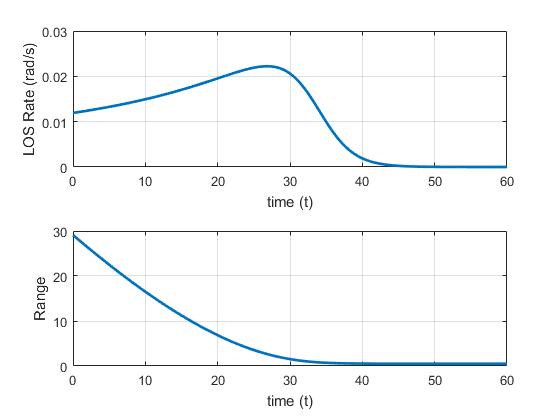
\includegraphics[width=7cm] {x15_range_LOSrate}
	\caption{Successful follow LOS-rate and range}
	\label{fig:successfulFollowLOS}
		\hspace*{0mm}
\end{figure}



\subsection{Intercept and Follow Model}
The LOS rate and range uncertainties in $x$ and $y$ are assumed to be equal, therefore the actual position of the target is in the space $(x_T\pm r,y_T \pm r)$, where $r$ is the radius of uncertainty. Figure \ref{fig:uncertrad} shows a representation of the measurement as a point centered in a circle of radius $r$. The region inside the circle is the space where the target may actually exist. The interceptor should avoid the inside of the circular region to prevent an unintended collision with the target. The uncertainty decreases linearly as a function of range as shown in Equations \ref{eq:uncert} and \ref{beq}.

\begin{figure}[H]
	\centering
	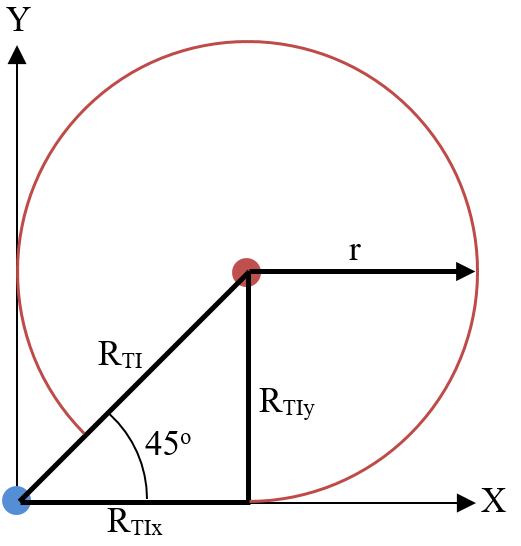
\includegraphics[width=4cm]{45deguncert.PNG}
	\caption{Position uncertainty radius centered on target}
	\label{fig:uncertrad}
\end{figure}




\begin{equation} \label{eq:uncert}
r = dr \,\sqrt[]{(x_T - x_I)^2+(y_T - y_I)^2}+b
\end{equation}




\begin{equation} \label{beq}
b = r_0-dr \,\sqrt[]{(x_{T0} - x_{I0})^2+(y_{T0} - y_{I0})^2}
\end{equation}

Sensing of range and direction was modeled as a function of the range $R_{TI}$, rate of change $dr$, and the minimum uncertainty radius $b$. A pseudotarget was introduced into the engagement scenario which prevents the interceptor from entering the region of uncertainty while maintaining the requirements of intercepting and following the target. The modified guidance was developed to satisfy a small range of scenarios where the target travels at constant heading, altitude, and speed equal to that of the interceptor. The interceptor avoids the region of uncertainty while following and intercepting the target by pursuing a pseudotarget. 



The pseudotarget acted as a state machine consisting of $wait$, $intercept$, and $follow$ states shown in Figures \ref{fig:wait}, \ref{fig:intercept}, and \ref{fig:follow} respectively. When the minimum altitude of the uncertainty is below the horizon $y_I-r<0$ the pseudotarget's state is set to $wait$ and waits at it's current position. Uncertainty decreases as the target approaches the interceptor eventually satisfying the condition $y_I-r >0$ triggering a change in state from $wait$ to $intercept$. When the $intercept$ state is active the pseudotarget is placed at the minimum uncertainty $y=y_T-r$ with no movement in the $x$ axis, $x=0$. Placing the pseudotarget at the minimum uncertainty altitude prevents the possibility of an unintended collision with the target. Intercept is intended to reduce the range to the target and get close, but not result in a collision. Once $x_T<x_I$ the problem becomes a tail chase scenario and the risk of collision is non existent. The algorithm is set to the $follow$ state where the pseudotarget is placed on top of the targets estimated position. 



\begin{figure}[H]
	\centering
	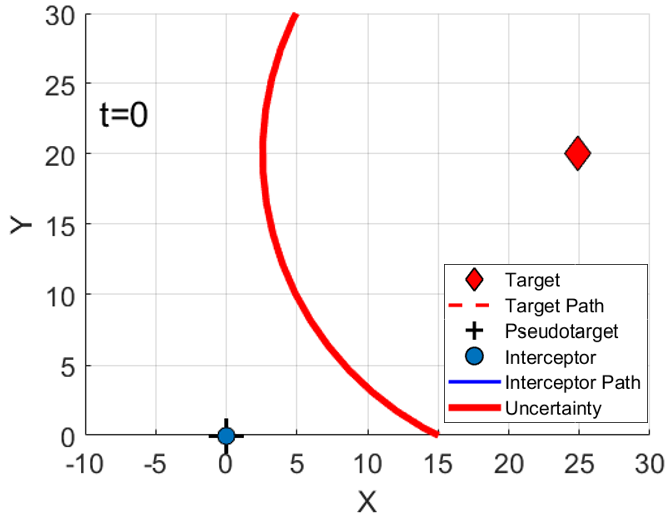
\includegraphics[width=7cm]{wait}
	\caption{Uncertainty below the horizon sets pseudotarget state to wait}
	\label{fig:wait}
\end{figure}

\begin{figure}[H]
	\centering
	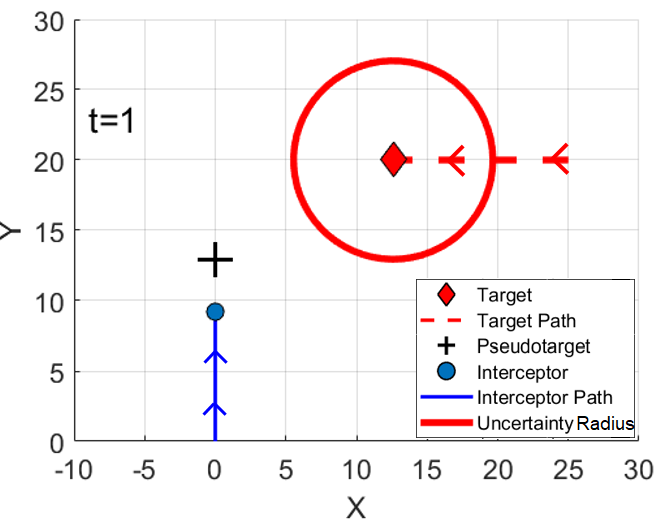
\includegraphics[width=7cm]{intercept}
	\caption{Uncertainty above the horizon sets pseudotarget state to intercept}
	\label{fig:intercept}
\end{figure}

\begin{figure}[H]
	\centering
	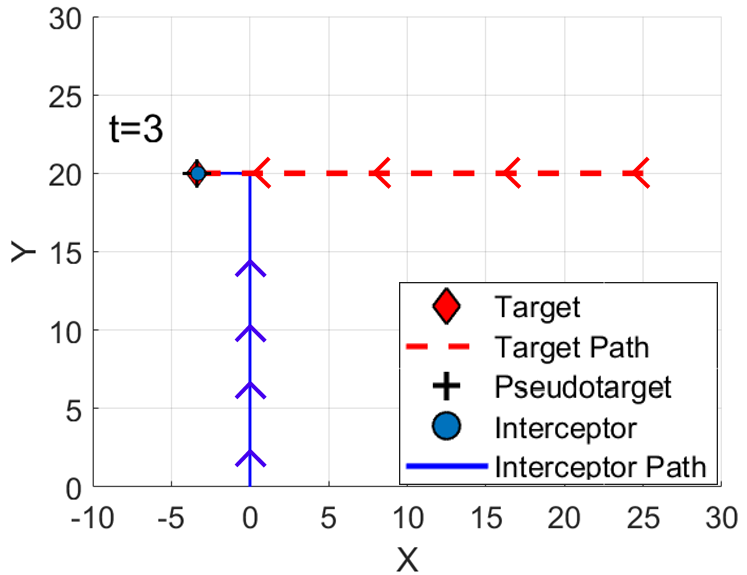
\includegraphics[width=7cm]{follow}
	\caption{Target estimate $x_T < 0$ sets pseudotarget state to follow}
	\label{fig:follow}
\end{figure}



With the target moving at constant altitude and both vehicles sharing the same velocity, it is expected that the following distance will be near zero if the intercept is active when $x_T \geq y_T$. If the intercept occurs when $x_T<y_T$, the interceptor is at a disadvantage and will fail to close the distance. The sensor was modeled so that the uncertainty circle is above the horizon once the target has crossed the $x=y$ line by calculating an appropriate initial uncertainty $r_0$. Referring back to Figure \ref{fig:uncertrad} a target at a LOS of $45^{\circ}$, has an altitude of $R_{TIy}$, and an initial uncertainty radius $r_0$. Determining the initial radius was done geometrically in Equations \ref{minr} and \ref{rtiforminr} and was set to $0.7$ times the initial range.



\begin{equation} \label{minr}
\sin(45^\circ) = \frac{y_T - y_I}{\sqrt[]{(x_T - x_I)^2+(y_T - y_I)^2}}
\end{equation}



\begin{equation} \label{rtiforminr}
 (y_T - y_I) = \sqrt[]{(x_T - x_I)^2+(y_T - y_I)^2}\sin(45^\circ)
\end{equation}



\begin{equation} \label{initialr}
r_0 = 0.7R_{TI}
\end{equation}

The impact of $r_0$ on following distance can be seen in Figures \ref{fig:rti07} and \ref{fig:rti08}.
 Each Figure shows the results of three target initial conditions along the $x=y$ line. Figure \ref{fig:rti07} shows a near zero following distance for a $r_0$ ratio of $0.7R_{TI}$. When $r_0>0.7R_{TI}$ the following distance becomes less predictable and is not constant along the target initial conditions on the $x=y$ line as shown in Figure \ref{fig:rti08}.
 


\begin{figure}[H]
	\centering
	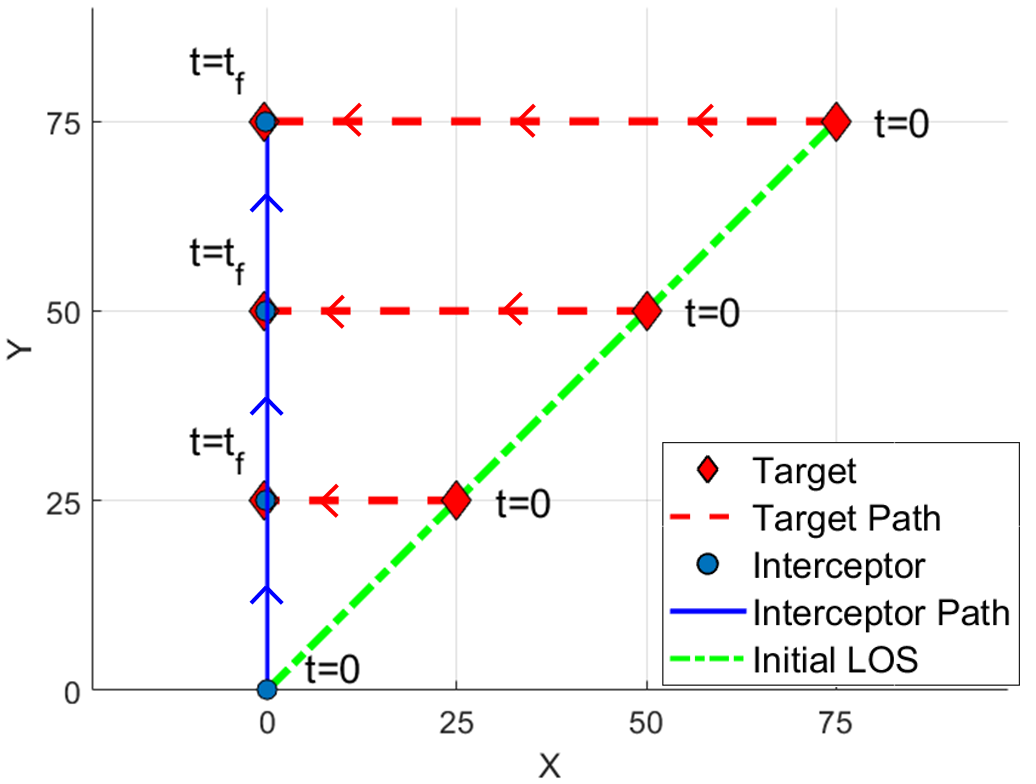
\includegraphics[width=7cm]{Rinit07new.png}
	\caption{Initial uncertainty ratio $0.7R_{TI}$ results in consistent following distance}
	\label{fig:rti07}
\end{figure}

\begin{figure}[H]
	\centering
	\includegraphics[width=7cm]{rinit08new.png}
	\caption{Initial uncertainty ratio $>0.7R_{TI}$ results in increasing following distance as initial range increases}
	\label{fig:rti08}
\end{figure}




The modified pseudotarget PN guidance was given the same initial conditions as shown in Figure \ref{fig:failedIntercept} and the performance compared. Traditional PN guidance performed well during the tail-chase but failed to follow the target and experienced a LOS singularity for a head-on intercept. The PN guidance with a psuedotarget successfully intercepts and follows the target, Figure \ref{fig:modifiedPNsuccess}, with non-singularity LOS rates, shown in Figure \ref{fig:modifiedPNsuccessLOS}. Traditional PN out performed the pseudotarget PN guidance for target initial condition $x_{T} = 15$ which demonstrates that a single guidance algorithm may not be suitable for all cases and a decision on which algorithm to use for a given set of initial conditions should be made. Table \ref{my-label} summarizes the performance of the algorithms for the two initial conditions.


\begin{figure}[H]
	\centering
	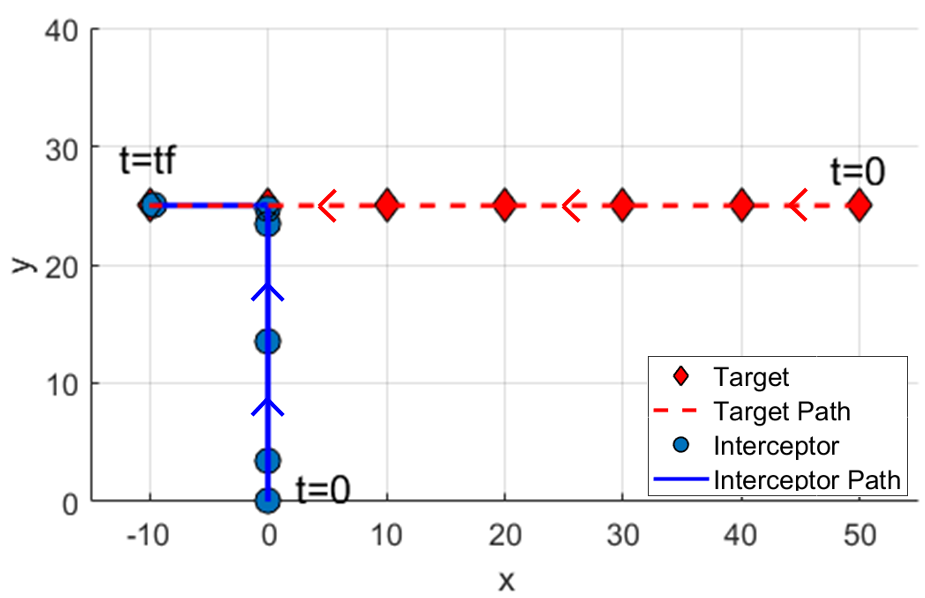
\includegraphics[width=7cm] {fixedSingularity}
	\caption{Tail chase with no singularities, and steady state range $R_{TI}\approx0$}
	\label{fig:modifiedPNsuccess}
	\hspace*{0mm}
\end{figure}

\begin{figure}[H]
	\centering
	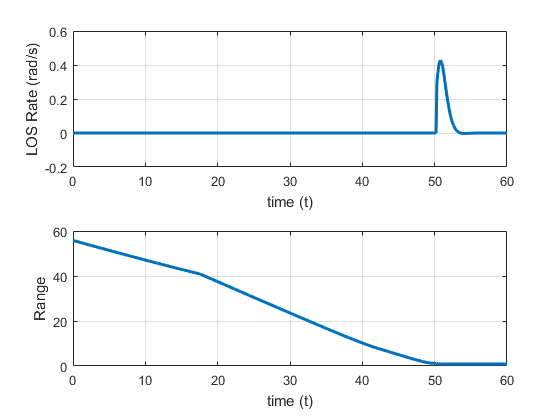
\includegraphics[width=7cm] {ptx50_range_LOSrate}
	\caption{Tail chase with no singularities, and steady state range $R_{TI}\approx0$}
	\label{fig:modifiedPNsuccessLOS}
	\hspace*{0mm}
\end{figure}



\begin{table}[H]
	\centering
	\caption{Traditional PN and Pseudotarget PN Following Distance and LOS rate}
	\label{my-label}
	\begin{tabular}{c|c|c|}
		\cline{2-3}
		\multicolumn{1}{l|}{}                                        & \multicolumn{1}{l|}{Following Distance} & \multicolumn{1}{l|}{Max LOS Rate (rad/s)} \\ \hline
		\multicolumn{1}{|c|}{}                                       & 0.51                                    & 0.02                                      \\ \cline{2-3} 
		\multicolumn{1}{|c|}{\multirow{-2}{*}{Traditional PN}}       & \cellcolor[HTML]{C0C0C0} FAILED         & 46.07                                     \\ \hline
		\multicolumn{1}{|c|}{}                                       & 6.51                                    & 0.06                                      \\ \cline{2-3} 
		\multicolumn{1}{|c|}{\multirow{-2}{*}{PN with Pseudotarget}} & 0.88                                    & 0.04                                      \\ \hline
	\end{tabular}
\end{table}

\section{Simulations}
The pseudotarget state machine PN guidance was validated through MATLAB simulations and a ratio for predicting following distance as a function of initial LOS, range, and sensor characteristic is presented for a non maneuvering target. Initial target conditions of $x = [-100,100]$ $y = [10,100]$ in $1$ unit increments were evaluated with a constant heading of $\beta = 180^{\circ}$. Initial uncertainty radius of the target estimate for each scenario was $0.7$ times the initial range with rate of change $dr = 1$. Interceptor initial conditions remained constant where the initial position and heading were $(0,0)$ and $90^{\circ}$ respectively. Each UAV was given the same velocity so that the speed ratio of the two vehicles was 1:1. When the interceptor's heading $\gamma = \beta$ the simulation was terminated and the final positions of the vehicles recorded. Dividing the following distance by the initial range to the target produces a following distance initial range ratio $\zeta$, shown in Equation \ref{eq:FDIR} which can be used to describe the performance of the model.


\begin{equation} 
\label{eq:FDIR}
\zeta = \sqrt{\frac{(x_{Tf}-x_{If})^2+(y_{Tf}-y_{If})^2}{(x_{T0}-x_{I0})^2+(y_{T0}-y_{I0})^2}}
\end{equation}

The unit-less $\zeta$ ratio in the simulation space is shown in the contour plot Figure \ref{fig:Rays}. Each target initial condition corresponds to a FDIR ratio on the plot, ranging from $0$ to $1.65$. $\zeta$ is constant along each initial LOS which allows for the prediction of following distance based on initial LOS, range, and sensor $dr$. Initial LOS angles less than $45^{\circ}$ yield a $\zeta$ ratio of near zero indicating that the following distance was near zero. Increasing LOS angles greater than $45^{\circ}$ result in progressively higher $\zeta$ ratios indicating an increasing following distance.



\begin{figure}[H]
	\centering
	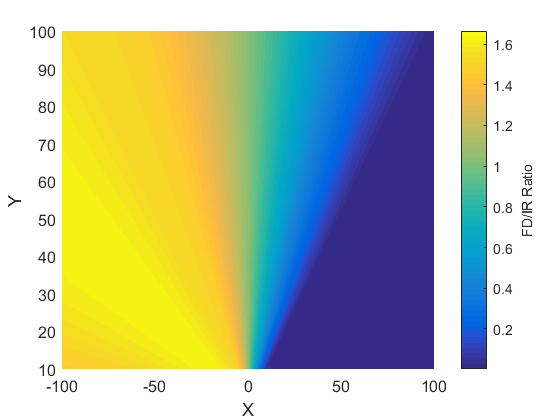
\includegraphics[width=8cm]{FDIR_Rays.png}
	\caption{Following distance to initial range ratio constant along each initial LOS}
	\label{fig:Rays}
\end{figure}

Representation of the models performance for a range of sensor $dr$'s is shown in Figure \ref{fig:Polar}. Simulations were performed for initial LOS angles ranging from $0^{\circ}$ to $180^{\circ}$ and sensors with $dr$ ranging from $0.5$ to $1$ in $0.5^{\circ}$ and $0.01$ unit increments respectively. Sensors with $dr < 0.5$ would not allow the interceptor to reduce the following distance much farther than the initial range for nearly all LOS angles. Sensors with $dr \geq 1$ the following distance can be reduced to nearly zero for initial LOS angles between $0$ and $45^{\circ}$. 

\begin{figure}[H]
	\centering
	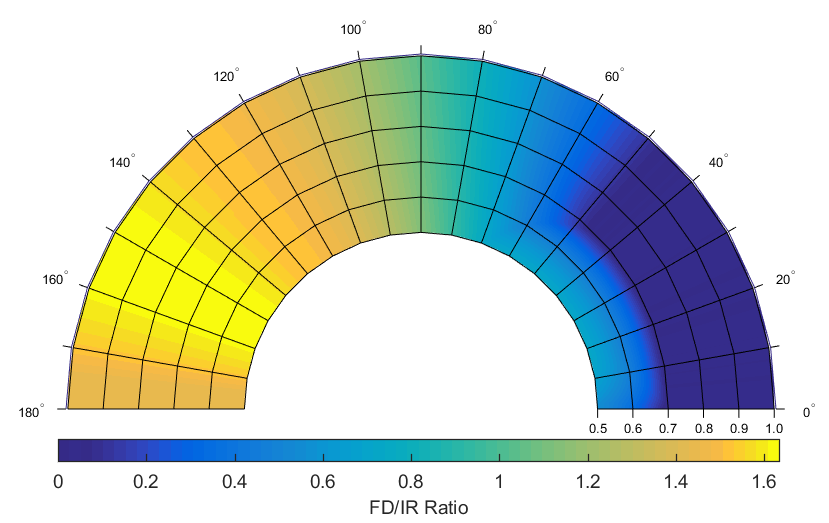
\includegraphics[width=8cm]{correctpolar.png}
	\caption{Following distance to initial range ratio for multiple sensor $dr$ confirm predicted near zero following distance for initial LOS $\leq45^\circ$}
	\label{fig:Polar}
\end{figure}

\section{Conclusion}



A pseudotarget based proportional navigation (PN) guidance algorithm that directs a UAV to intercept and follow a target UAV using highly uncertain sensor position information was investigated. Simulations were performed to determine the following distance for a finite space. Near zero following distance was achievable for a finite range of initial headings and sensor $dr$'s. Following distance to initial range ratios indicate that the modified guidance performs optimally when the initial LOS angle is less than $45^\circ$ and larger initial sight angles may benefit from other intercept methods. The state machine pseudotarget PN guidance algorithm was specifically designed to intercept and follow an inbound non-maneuvering target for the edge case of $1:1$ speed ratio. Initial results suggest that the proposed guidance is tracks the target with less error compared to traditional PN for head-on intercepts but slightly underperformed in the tail-chase scenario.




\section{Acknowledgements}
The research presented was funded by Wright-Patterson Air Force Research Laboratory under SFFP . 



\bibliographystyle{IEEEtran}
\bibliography{bib}

\end{document}


